% Latex template: mahmoud.s.fahmy@students.kasralainy.edu.eg
% For more details: https://www.sharelatex.com/learn/Beamer

\documentclass{beamer}					  % Document class

\usepackage[portuguese]{babel}			  % Set language
\usepackage[utf8x]{inputenc}			  % Set encoding

\mode<presentation> {					  % Set options
  \usetheme{default}					    % Set theme
  \usecolortheme{default} 				% Set colors
  \usefonttheme{default}  				% Set font theme
  \setbeamertemplate{caption}[numbered]	% Set caption to be numbered
}

\setbeamertemplate{navigation symbols}{}
\setbeamertemplate{footline}[frame number]
\setbeamercovered{transparent}

% Uncomment this to have the outline at the beginning of each section highlighted.
%\AtBeginSection[]
%{
%  \begin{frame}{Outline}
%    \tableofcontents[currentsection]
%  \end{frame}
%}

\usepackage{graphicx}					% For including figures
\usepackage{booktabs}					% For table rules
\usepackage{hyperref}					% For cross-referencing
\usepackage{caption}                    % Allows more control over captions in figs and tables

\title{Revisão de Atividades da FAC}	% Presentation title
%\author{Author One}					% Presentation author
\institute{LNLS.DAC.FAC}				% Author affiliation
\date{2024-02-16 -- 2024-03-08}			% Today's date	


\begin{document}



\begin{frame}
  \titlepage
  \href{https://github.com/lnls-fac/doc-review-dac-fac}{\beamergotobutton{Link para o repo github desta apresentação: https://github.com/lnls-fac/doc-review-dac-fac}}
  \href{https://www.overleaf.com/read/sbdjxtzfchrm}{\beamergotobutton{Link para o projeto overleaf destas notas}}
\end{frame}

\begin{frame}{Outline}
  \tableofcontents
\end{frame}




% \section{CBI Transversais}

% \begin{frame}{CBI Transversais}
%     \scriptsize{\begin{itemize}
%             \item Estudo de máquina 29/01, BbB
%     \end{itemize}}
%     \begin{figure}[H]
%         	\centering
%             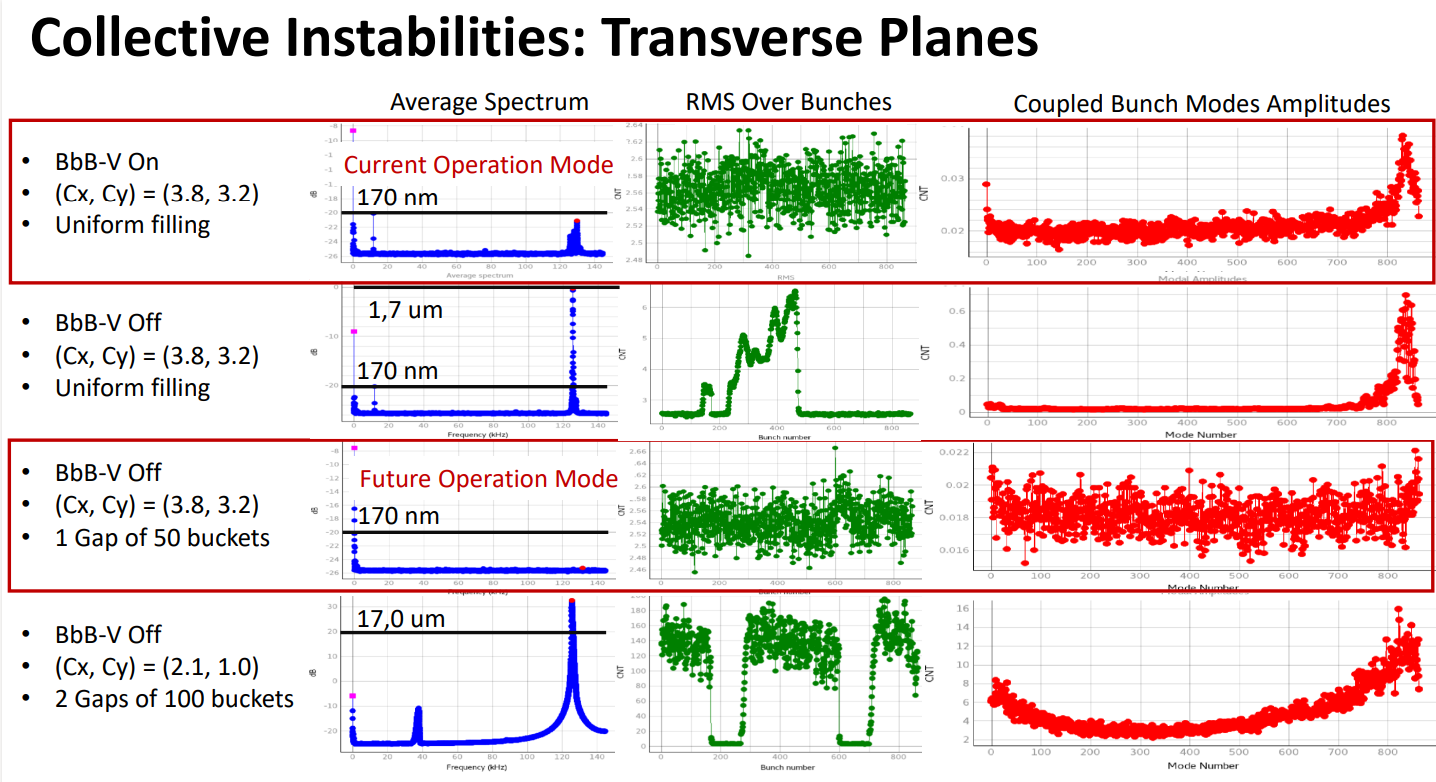
\includegraphics[width=1.0\textwidth]{2024-03-08/figures/cbi-transversais.png}
%             \label{fig:cbi-transversal}
%     \end{figure} 
% \end{frame}



\section{NLK}

\begin{frame}{NLK}
    \vspace{0.2 cm}
    Experimento 2024-02-20
    \vspace{0.2 cm}
    \begin{itemize}
            \item Minimizado o pulso de kick NLK+HCoil mas não a perturbação no feixe distribuído (centróide).
    \end{itemize}
    \begin{columns}
        \begin{column}{0.75\textwidth}
            \begin{figure}[H]
                \centering
                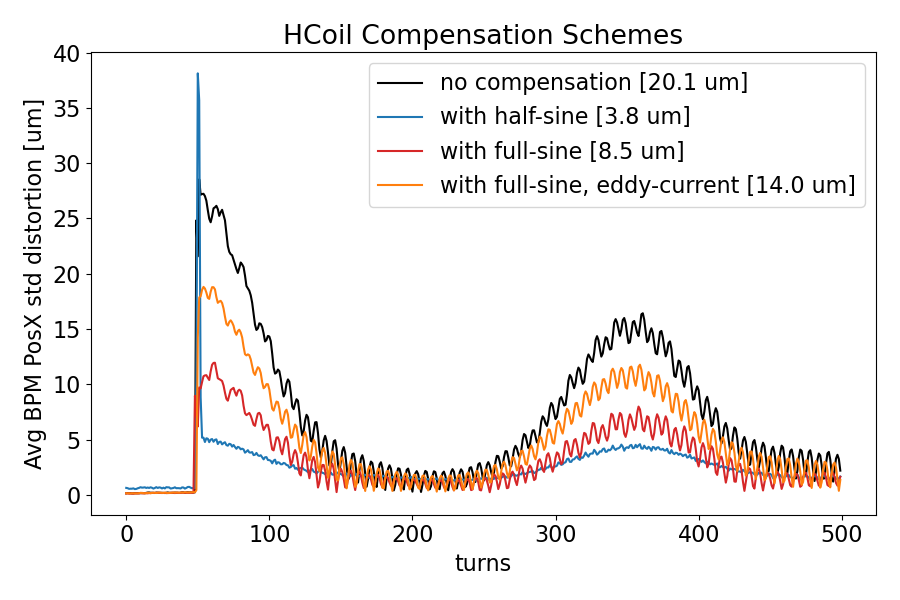
\includegraphics[width=1\textwidth]{2024-03-08/figures/hcoil-compensation-scheme.png}
                \label{fig:hcoil-distortion}
            \end{figure}
        \end{column}
        \begin{column}{0.4\textwidth}
            \begin{figure}[H]
                \centering
                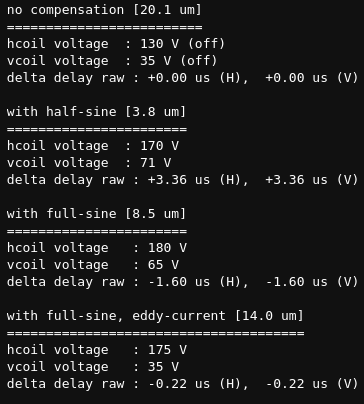
\includegraphics[width=1.0\textwidth]{2024-03-08/figures/hcoil-table.png} \hspace*{4cm}
                \label{fig:hcoil-table}
            \end{figure}
        \end{column}
    \end{columns}
\end{frame}


\begin{frame}{NLK}
    \vspace{0.2 cm}
    \begin{itemize}
            \item Kick do NLK no feixe localizado em função do atraso
    \end{itemize}
        \begin{figure}[H]
            \centering
            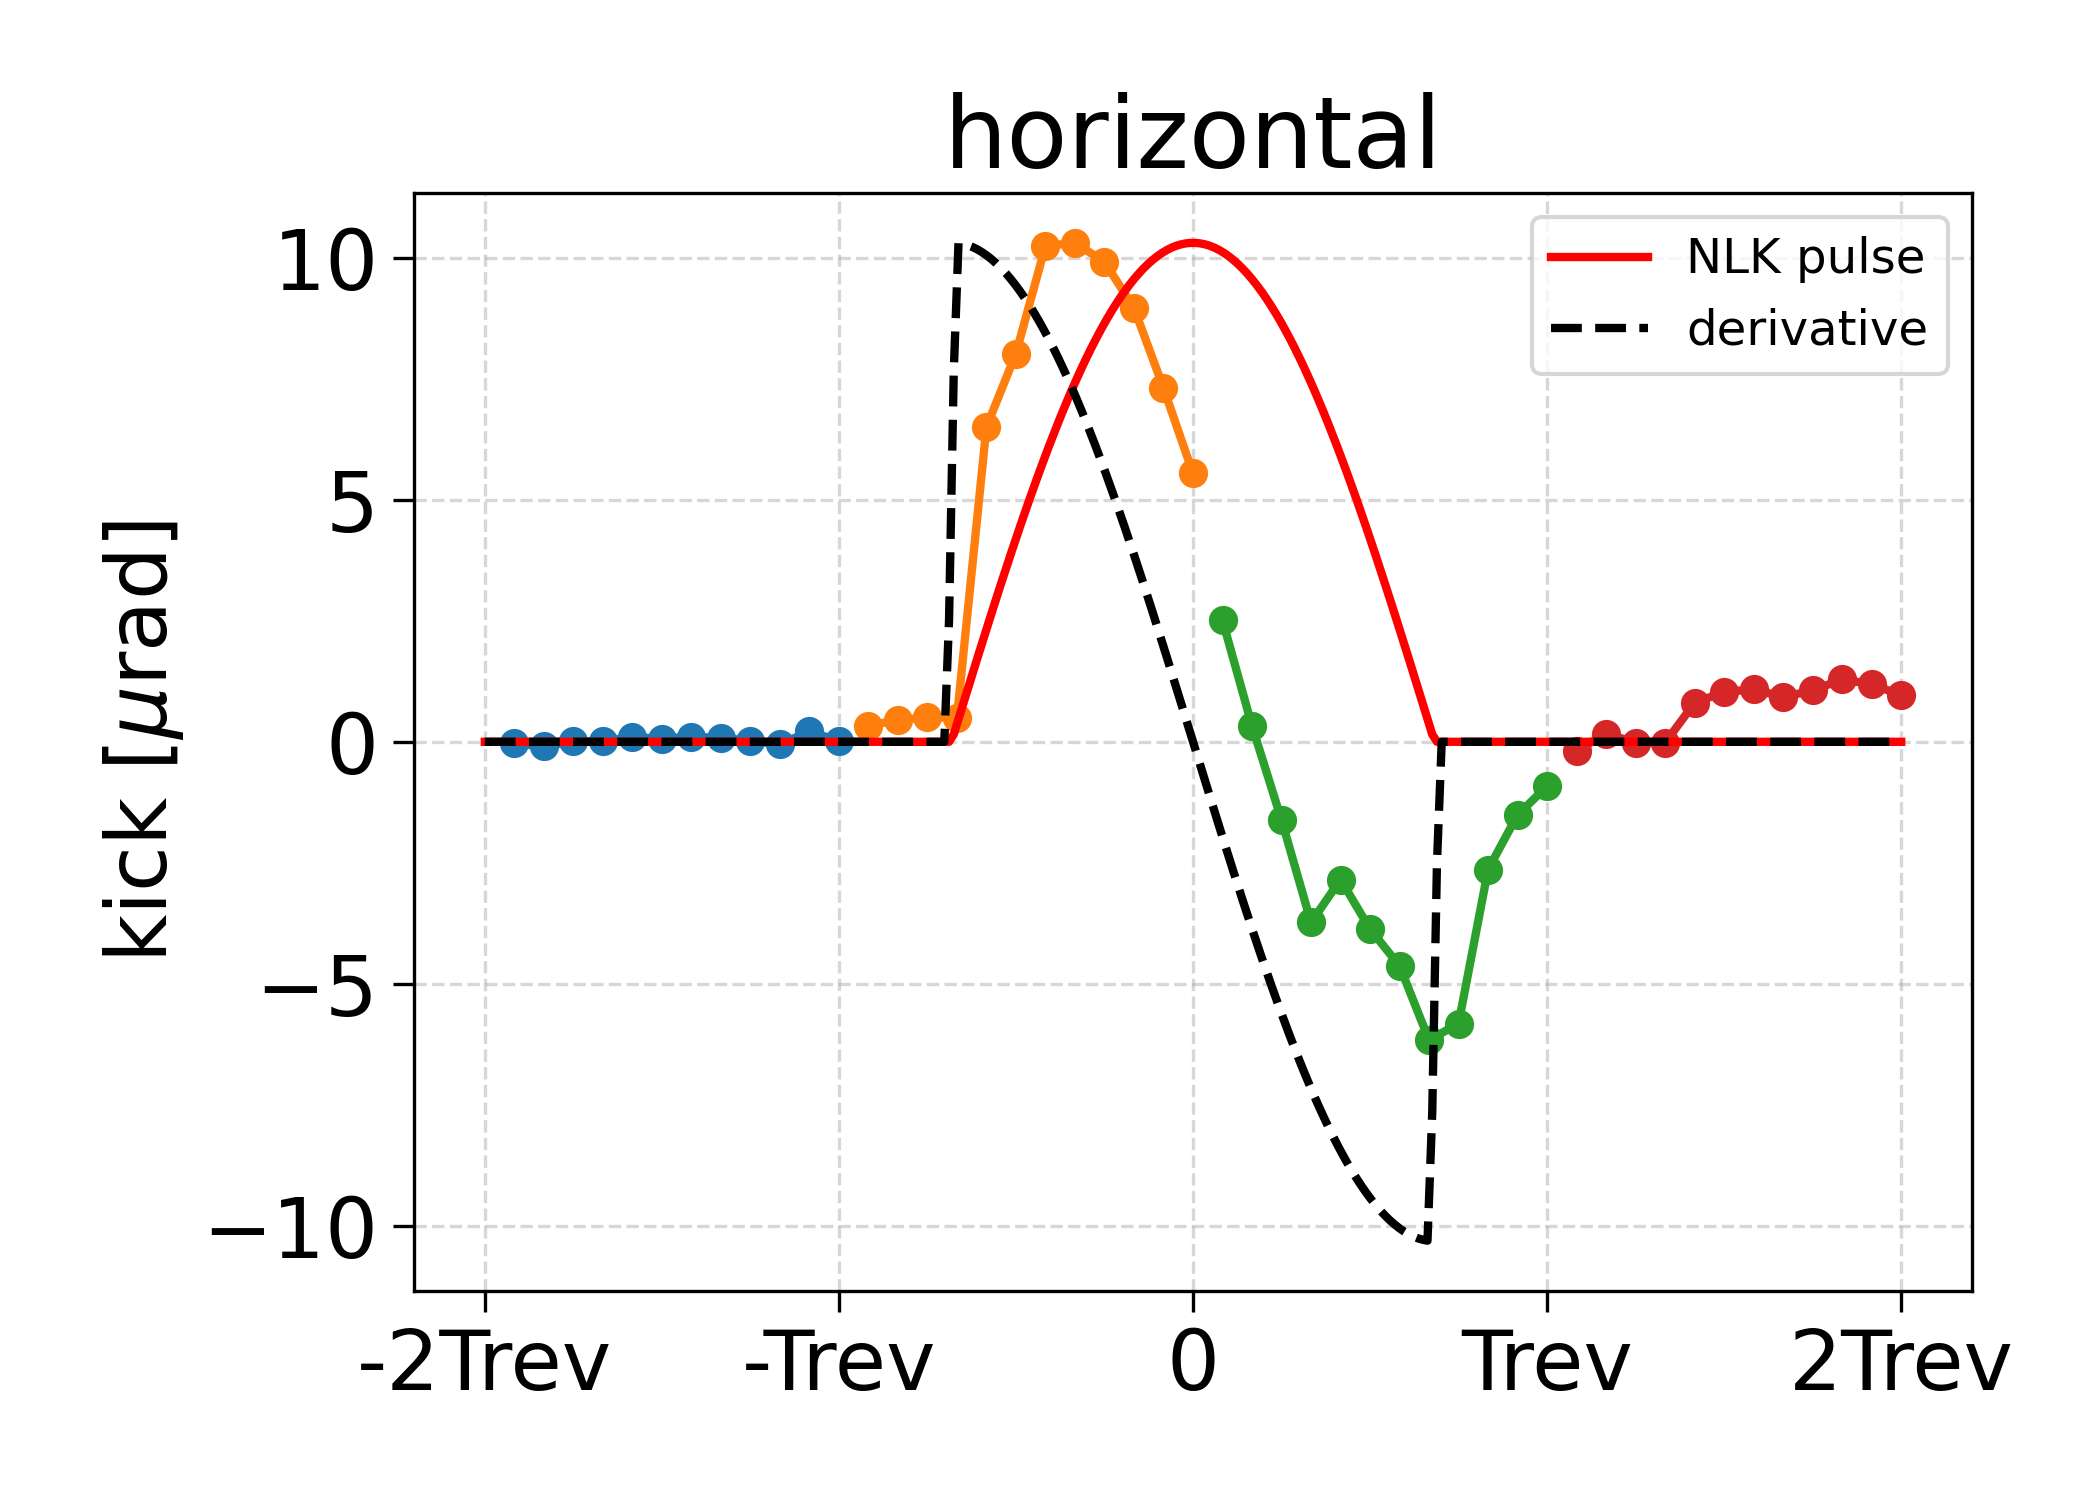
\includegraphics[width=1\textwidth]{2024-03-08/figures/hcoil-kick.png}
            \label{fig:hcoil-distortion}
        \end{figure}
\end{frame}


\section{Rampa do Booster}

\begin{frame}{Rampa do Booster}
    \vspace{0.4 cm}
    \large{
    \begin{itemize}
            \item BO flop $\rightarrow$ flip: correção da órbita ao longo de toda a rampa de energia também para o estado flop. (2024-02-27) \vspace{0.5cm}
            \item Forças QD e QF do flop (sintonias corrigidas) aplicadas à rampa flip. (usuários 2024-02-29)
    \end{itemize}
    }
\end{frame}



\section{Problemas Pendentes}

\begin{frame}{Problemas Pendentes}
    \vspace{0.4 cm}
    \large{
    \begin{itemize}
            \item Injeção ruim com PUs em stand-by ($\rightarrow$ desligado) \vspace{0.5cm}
            \item FB LLRF da P7Cav com $K_P$ e $K_I$ reduzidos. \vspace{0.5cm}
            \item FB de Field Flatness da P7Cav desligado por problema com os sinais de potência das células 2 e 6. (algumas questões na interface de controle da RF)
    \end{itemize}
    }
\end{frame}



\section{References}



\end{document}
